\documentclass[10pt,a4paper,oneside,fleqn]{report}
\usepackage{geometry}
\geometry{a4paper,left=20mm,right=20mm,top=1cm,bottom=2cm}
\usepackage[utf8]{inputenc}
%\usepackage{ngerman}
\usepackage{amsmath}                % brauche ich um dir Formel zu umrahmen.
\usepackage{amsfonts}                % brauche ich für die Mengensymbole
\usepackage{graphicx}
\setlength{\parindent}{0px}
\setlength{\mathindent}{10mm}
\usepackage{bbold}                    %brauche ich für die doppel Zahlen Darstellung (Einheitsmatrix z.B)
\usepackage[linktocpage={false}]{hyperref}


\usepackage{color}
\usepackage{titlesec} %sudo apt-get install texlive-latex-extra

\definecolor{darkblue}{rgb}{0.1,0.1,0.55}
\definecolor{darkred}{rgb}{0.55,0.2,0.2}

\titleformat{\chapter}[display]{\color{darkred}\normalfont\huge\bfseries}{\chaptertitlename\
\thechapter}{20pt}{\Huge}

\titleformat{\section}{\color{darkblue}\normalfont\Large\bfseries}{\thesection}{1em}{}
\titleformat{\subsection}{\color{darkblue}\normalfont\Large\bfseries}{\thesection}{1em}{}

% Notiz Box
\usepackage{fancybox}
\newcommand{\notiz}[1]{\vspace{5mm}\ovalbox{\begin{minipage}{1\textwidth}#1\end{minipage}}\vspace{5mm}}

\usepackage{cancel}


%\includegraphics[width=0.75\textwidth]{thepic.png}

\begin{document}
\tableofcontents
\setcounter{chapter}{11}
\chapter{Magnetismus}

Die Magnetisierung \(\vec M\) ist das magnetische Moment pro Volumen. \(\vec M = n\vec\mu\) ; \(\mu\) ist mittleres Dipolmoment.


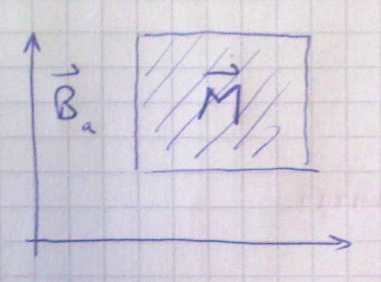
\includegraphics[width=0.75\textwidth]{kap12_01.png}


Magnetische Suszeptibilität: \([\chi]\) Tensor

\[[\chi]\equiv \chi = \frac{\vec M}{\vec H} = \mu_0\frac{\vec M}{\vec B} \]

Skalar (Vereinfacht) \(\chi= \frac{M}{H}\); \(\chi < 0 \): diamagnetische festkörper; \(\chi>0\): paramaggnetische Festkörper

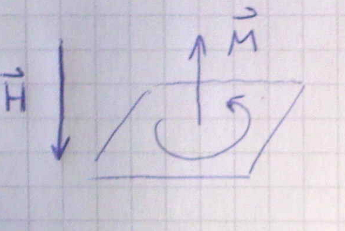
\includegraphics[width=0.75\textwidth]{kap12_02.png}


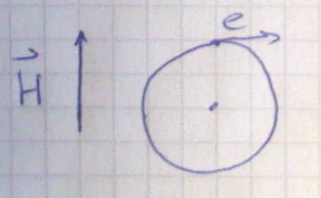
\includegraphics[width=0.75\textwidth]{kap12_03.png}


Lenz-Regel \(I \propto \frac{d\phi}{dt}\)

\section{Diamagnetismus}

Diamagnetismus ist eine Schwächung des äußeren Feldes. Klassische (Langevin) und quantenmechanische Behandlung. Beide kommen zu gleichen Resultaten. 




\[\left.\chi_d\right|_{\text{Atome}}\propto 10^{-6}\text{ bis }10^{-7}\]

\[\left.\chi_a\right|_{\text{Atome}} = -\frac{h\mu_0 e^2}{6m_e}Z \langle r^2\rangle \]

mit \(Z\) Elektronenzahl und \(\langle r^2\rangle  \) mittlerer abstandsquadrat der e-nen

\subsection{Diamagnetismus freier Elektronen: Landau-Diamagnetismus}

1930 Landau-Quantisierung \(\frac{\hbar(k^2_x+k^2_y)}{2m_e} = (l+\frac{1}{2})\hbar\omega_c\); \(l=0,1,2,3...\) B-Feld in z-Richtung.

mit \(\chi = -\frac{\partial^2 F}{\partial H^2}\)

\[F = k_B T ln\sum_{\text{alle Zustände}}e^{-\frac{iE}{k_B T}}\]

\[\left.\chi_d\right|_{\text{Landau}}= -\frac{1}{3}\mu_B^2\mu_0 D(E_F) =-\frac{1}{3}\mu_B^2\mu_0 \frac{3}{2}\frac{n}{E_F} = -\frac{n}{2E_F}\mu_0\mu_B^2 \propto 2\cdot 10^{-7} \]

mit dem Borsches Magneton \( \mu_B=\frac{e\hbar}{2m_e} \) und Zustandsdichte \(D(E_F) \)


\section{Paramagnetismus}

Paramagnetismus freier e-nen ist allgemein bekannt als Paulische Spin Suszeptibilität.

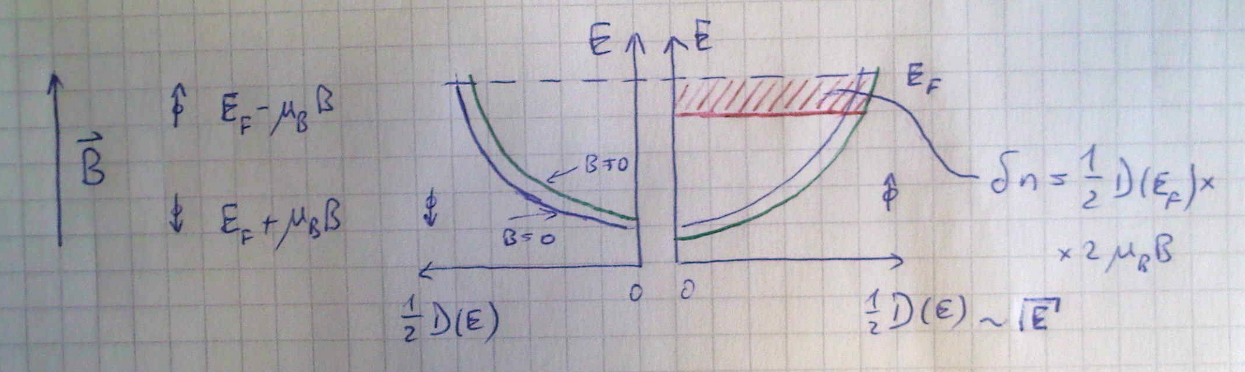
\includegraphics[width=0.75\textwidth]{kap12_04.png}

Roter Bereich \(\delta n\) kommt dazu, es gibt insgesammt mehr Elektronen

\[\delta n = \frac{1}{2}D(E_F) 2\mu_BB\]

\[M = \delta n \mu_B = \mu_B^2 B D(E_F)\]

\[\left.\chi_P\right|_{\text{Pauli}} =\mu_B\frac{M}{B} = \mu_0\mu_B^2 d(E_F) = \left.-3\chi_d\right|_{\text{Landauu}}\]

\[\boxed{ \left.\chi_P\right|_{\text{Landau}} = \left.-\frac{1}{3} \chi_d\right|_{\text{Pauli}} }\]


\subsection{Paramagnetismus von Ionen}

Aus der Atomphysik: \( \vec \mu = -g\mu_B\vec J'\) mit \(g\) Lande-Faktor \(\vec J'\hbar \vec J\) Gesamtdrehimpuls des Atoms

\[\hat J = \hat L + \hat S\]

\[g = 1 + \frac{J(J+1)+S(S+1)-L(L+1)}{2J(J+1)}\]

\(L\)-Bahndrehimpulsquantenzahl und \(S\)-Spinquantenzahl

Quantentheorie ( nur für Zwei-Niveau-Spinsystem)


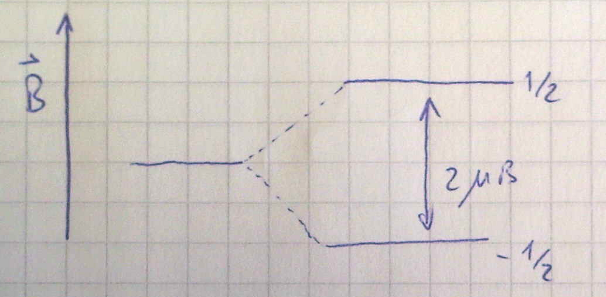
\includegraphics[width=0.75\textwidth]{kap12_05.png}

\[V = -\vec \mu\vec B = \underbrace{m_J g\mu_B}_{\mu} B\]

mit \(m_J=\pm\frac{1}{2}\); \(g=2\); \(V = \pm\mu_B B\)


Im Gleichgewicht für \(T\neq 0\); Faktor \(x=\frac{\mu B}{k_BT}\)

\[\frac{n_\uparrow}{n} = \frac{e^x}{e^x+e^{-x}}\]

\[\frac{n_\downarrow}{n} = \frac{e^{-x}}{e^x+e^{-x}}\]

Magnetisierung \(M=(n_\uparrow - n_\downarrow)\mu = n\mu tanh(x)\)

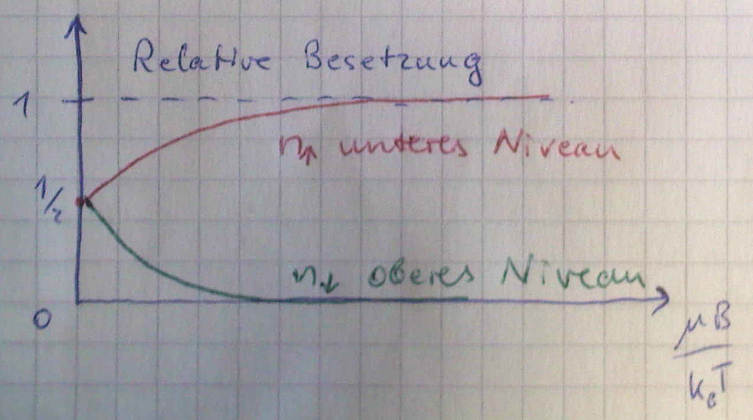
\includegraphics[width=0.75\textwidth]{kap12_06.png}

für \(x<<1\) (hohe T) \(tanh(x)\propto x\)

\[M\approx n\mu \frac{\mu B}{k_B T}\]

Curie-Gesetz:
\[\chi_{pa}\approx \frac{n\mu^2}{k_BT}\mu_0\approx \frac{1}{T}\]
Ein Atom mit Gesamtdrehimpulsquantenzahl J besitzt in einem Magnetfeld (2J+1) äquidistante Energieniveaus

\[M = ngJ\mu_B B_J(x)\]

mit \( B_J(x) \) Brillouin-Funktion für \(x<<1\)

\[\chi_{pi} = \mu_0\frac{\mu}{B} = n J(J+1)\frac{g^2\mu_B}{3k_BT}\propto\frac{C}{T}\]

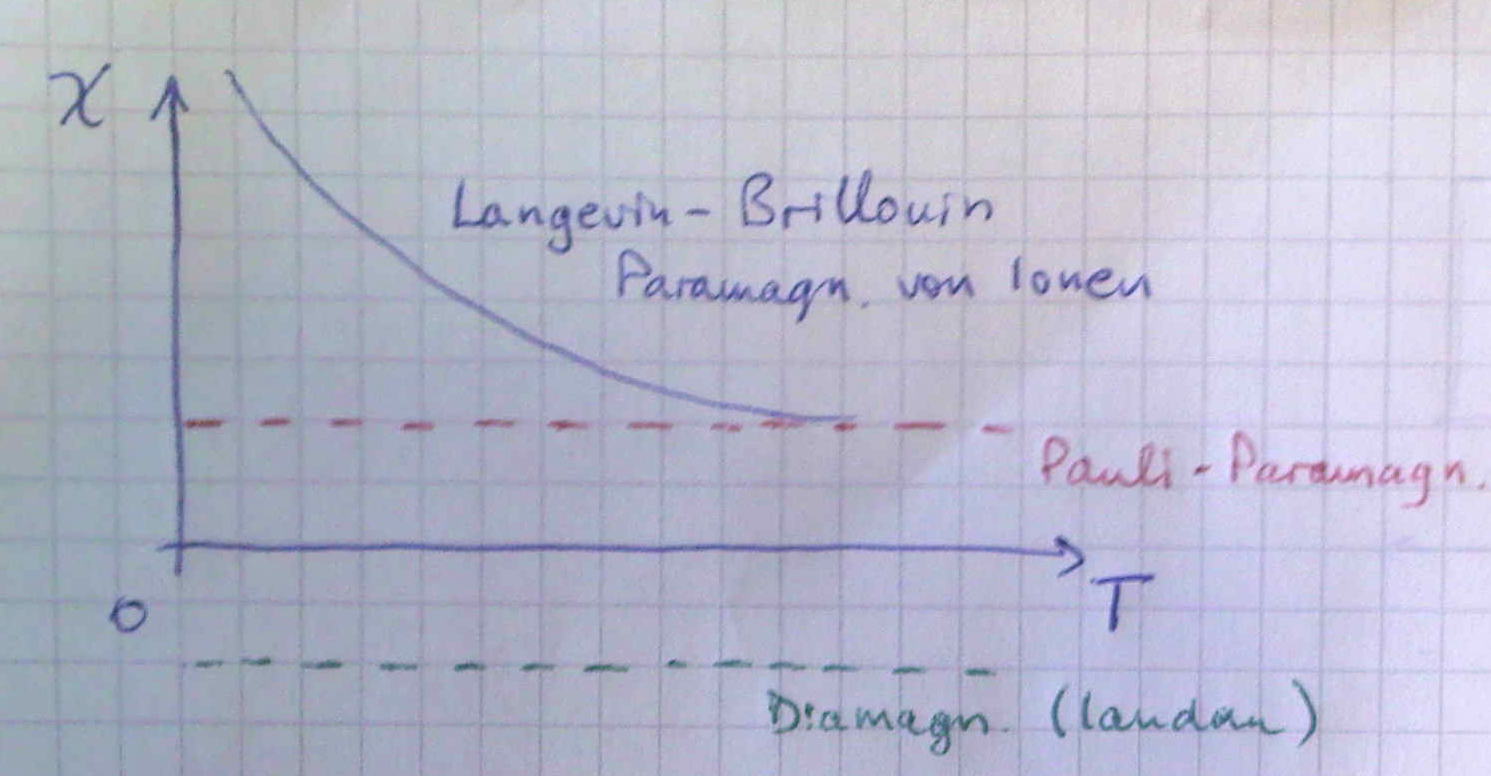
\includegraphics[width=0.75\textwidth]{kap12_07.png}

\section{Kühlung durch adiabatische Entmagnetisierung}

von Debye 1926 vorgeschlagen und 7 Jahre später realisiert.

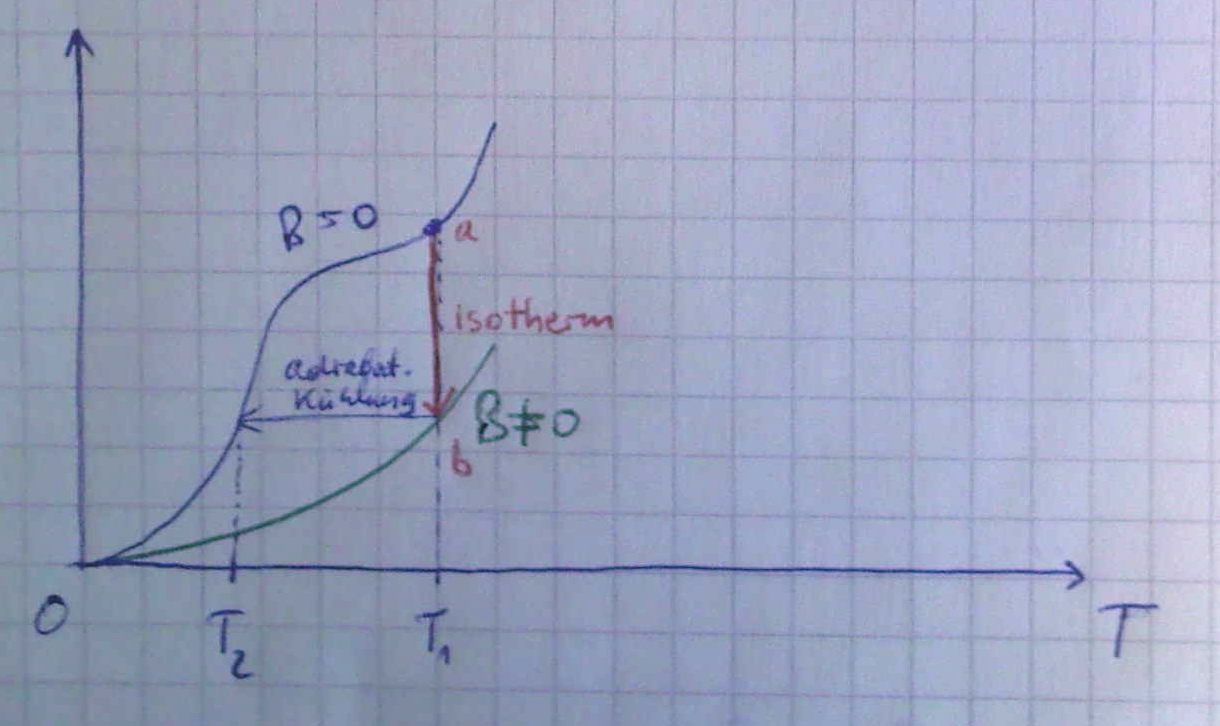
\includegraphics[width=0.75\textwidth]{kap12_08.png}

a - gute Wärmekontakt bis \(mK\)
b - Probe von Umgebung isoliert \(\approx 10 \mu K\) Bei Cu Kernentmagnetisierung



\section{Ferrormagnitismus}


\begin{itemize}
\item Spontante Magnetisierung unterhalb unterhalb einer kritischen Temperatur \(T_C\)
\end{itemize}
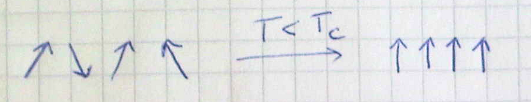
\includegraphics[width=0.75\textwidth]{kap12_09.png}

Grund: Energiegewinn durch Ausrichtung der magnetischen Momente

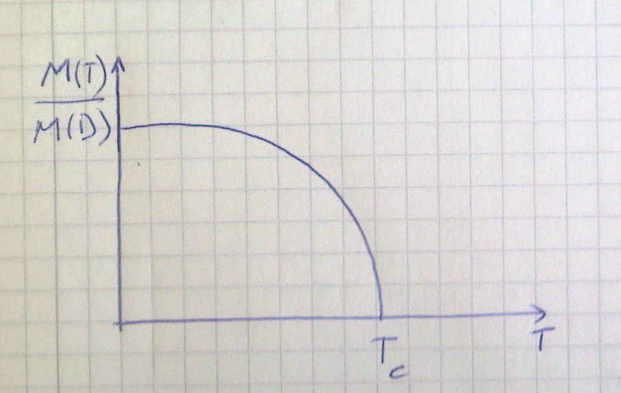
\includegraphics[width=0.75\textwidth]{kap12_10.png}



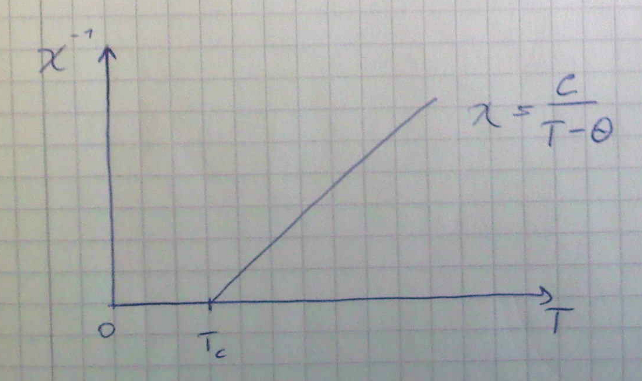
\includegraphics[width=0.75\textwidth]{kap12_11.png}



\begin{itemize}
\item[1)] Molekularfeldänderung
\end{itemize}
\[B_{eff}=B_A+B_H=B_a+\lambda\mu_0 M\]

\(\lambda\) ist die Molekularfeldkonstante mag WW für 2 Spinns: \(\approx 0.1 T\quad B_H\approx 1000T\)
\(\Rightarrow \) nicht durch die mag WW der Spins

Magnetisierung wird durch Molekularfeld getrieben

\[M_S = ng\mu_B J B(x),\qquad x = \frac{g\mu_B \lambda\mu_0 M_S}{k_B T}\]

Curie-Konstante
\[T_C = \frac{n g^2 J(J+1)\mu_B^2 \lambda}{k_B} = C\cdot\lambda\]

\[\Theta =\lambda\cdot C\]

mit \(\Theta\) paramagn Curie Temp.

Fe: \(\lambda\approx 5000,\quad M_S = 1,6\cdot 10^{6}\frac{A}{m}\qquad B_M \approx 1000T\)

\[p^2 = g^2 s(s+1)\]

\begin{itemize}
\item[2)] Austausch WW zwischen lokalen orten Elektronen
\end{itemize}

System 2 weiterer Ionen mit 2E (Isolator)

\[\psi(r_1,s_1;r_2,s_2) = \psi(r_1,r_2)\psi(s_1,s_2)\]

\[\psi_S = A[\psi_a(r_1) \psi_b(r_2)+\psi_b(r_1)\psi_a(r_2)  ]\]

Symmetrische Ortswellenfunktion \(\Rightarrow \) Spin Wellenfkt antisymmetrisch

\[\psi_A = A[\psi_a(r_1) \psi_b(r_2)-\psi_b(r_1)\psi_a(r_2)  ]\]

Antisymmetrische Ortswellenfunktion \(\Rightarrow \) Spin Wellenfkt symmetrisch

WW Potential des Gesamtzustandes

\[V(r_1,r_2) = \tilde V(r_2,r_1)\]

Austauschkonst J

\[ J = E_S - E_A \approx 4 A^2 \int \psi_a^*(r_1)\psi_b^*(r_2)\tilde V(r_1,r_2)\psi_b(r_1)\psi_a(r_2)dV_1dV_2\]

Kinetische Energie des e-trons wird vernachlässigt

\begin{itemize}
\item \(J>0\) - parallele Ausrichtung des Spins
\item \(J<0\) - antiparallele Ausrichtung des Spins
\end{itemize}

\[|J| = \frac{3k_B \Theta}{z s(s+1)}\]


\[\tilde V_{el}(r_1,r_2) = \frac{e^2}{(4\pi \epsilon_0|r_1-r_2|}\]

Coulomb WW versucht die Spins auszurichten. \(V_i(r_1,V_i(r_2)\), attraktiv, negative Beitrag zu J

relative Gröpe entscheidet über Ausrichtung der Spins

\underline{Alternativ} Pauliprinzip

\(S_1,S_2\) Spinoperatoren der Elektronen

\[S = |s_1+s_2|^2 = \frac{3}{2}+2s_1s_2\]

\(s_1s_2 = -\frac{3}{4}\) \(S=0\) Singulett Zustand
\(s_1s_2 = -\frac{1}{4}\) \(S=1\) Triplett Zustand

Hamilton Operator für Zustand Spin System

\begin{align}
H_{\text{spin}}&=\frac{1}{4}(E_S+3E_A)-(E_S-E_A)s_1s_2 \\
&=\underbrace{\frac{1}{4}(E_S+3E_A)}_{=0\quad \text{bei geeigneter Wahl des Nullpunktes}}-Js_1s_2 \\
&= -J_{ij}s_is_j\qquad |\text{Heisenberg Modell des Ferrormagneten}
\end{align}

\begin{itemize}
\item[3)] Austausch WW im freien Elektronen Gas
\end{itemize}

Freies Elektronengas \(\rightarrow \) Übergang Ebener Wellen

\begin{align}
\psi(r_1,r_2) &= A\left[e^{ik_1r_1}e^{ik_2r_2}- e^{ik_1r_2}e^{ik_2r_1}  \right]\\
&=Ae^{i(k_1r_1+k_2r_2)}\left[1-e^{ik(k_1-k_2)(r_1-r_2)}\right]
\end{align}

Aufenthaltswahrscheinlichkeit \(dV_1dV_2\)

\[|\psi(r_1,r_2)|^2dV_1dV_2 = |A|^2 \left[1-cos(k_1-k_2)(r_1-r_2)\right]\]

Die Wahrscheinlichkeit zwei Spins mit gleichen Spin am gleichen Ort zu finden verschwindet auch ohne Coulomb WW

\underline{Austauschloch}

Wenn Spins ausgerichtet sind, verringern sich die Abschirmeffekte der Ionenrümpfe und die Aufelektronen werden daher stärker gebunden. Es führt zu einem Energiegewinn.


\begin{itemize}
\item[3)] Spinwellen (Magnonen)
\end{itemize}


Niederenergetische Anregungen, ähnlich Phononen. Eine kollektive Anregung der Bewegung

Spinflip kostet \(\delta E = 2zJs^2; \qquad J\approx k_BT_C\)

Magnonen haben \(E = \hbar\omega\)

Ausrichtung in z-Richtung. Drehmoment \(\mu\times B_M = - g\mu_B S_M\times B_M\)

\[\frac{dS}{dt} = -g\mu_B S\times B_M\]

zeitliche Ableitung des Drehimpulses \(\hbar S =\) angreifenden Drehmoment.

\[U_m = -J S_m(S_{m-1}+S_{m+1}) = \mu B_M = g\mu_BS_MB_M\]

\[\frac{dS_M}{dt}= \frac{J}{\hbar}S_M\times (S_{m-1}+S_{m+1})\]

\[S_{m,x} = Acos(mqa-\omega t)\]
\[S_{m,y} = Asin(mqa-\omega t)\]
\[S_{m,z}\sqrt{S^2-A^2}\]


mit \(q= \frac{n\pi}{L}\) und \(L\) als die Länge der Kette

Dispersionsrelation

\[\omega = \frac{2JS}{\hbar}[1-cos(qa)] =\frac{4JS}{\hbar} sin^2(\frac{ga}{2}) \]

\[\omega = \frac{JS}{\hbar}a^2q^2\]

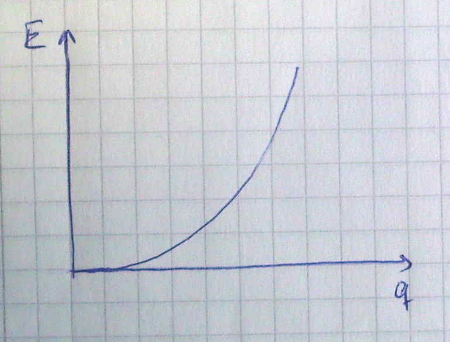
\includegraphics[width=0.75\textwidth]{kap12_12.png}


\end{document}
